\documentclass[11pt,a4paper]{article}
\input{../../sablony/pripravy/priprava.sty}
\usepackage{tikz}
\nastavPripravu{1. ročník}{Souhrnné opakování}{132}{Funkce vyprávějí příběh}
\begin{document}
\blok{Úvod a připomenutí}
Opakujeme tabulku, graf, předpis, definiční obor a obor hodnot lineární, kvadratické a absolutní funkce. Když je graf popisem skutečné situace, nemá automaticky definiční obor $\mathbb R$. Ve výpočtech zapisuj i jednotky a význam průsečíků.
\blok{Společně řešené příklady}
\begin{prikladReseniBox}[title={Příklad 1}]
Robot jede po přímé chodbě: první 2 minuty rychlostí $3\,\mathrm{m/min}$ od startu, další minutu stojí a pak se vrací rychlostí $2\,\mathrm{m/min}$. Zapište vzdálenost od startu $s(t)$ pro $0\le t\le6$ a určete $s(4)$ a obor hodnot.
\tcblower
\[
\begin{aligned}
s(t)&=\begin{cases}3t,&0\le t\le2,\\6,&2<t\le3,\\6-2(t-3),&3<t\le6,\end{cases}\\
s(4)&=6-2=4\,\mathrm m\\
H(s)&=\langle0;6\rangle\,\mathrm m
\end{aligned}
\]


\begin{center}
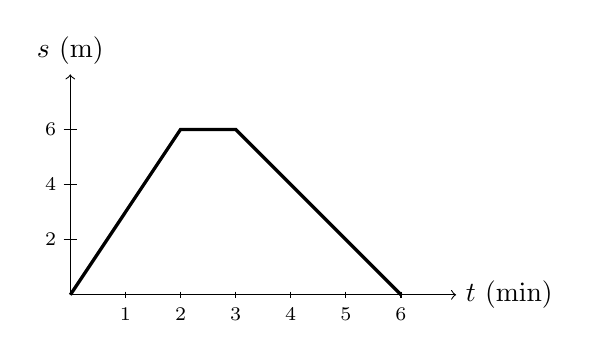
\begin{tikzpicture}[x=0.7cm,y=0.35cm]
\draw[->] (0,0)--(7,0) node[right] {$t$ (min)};
\draw[->] (0,0)--(0,8) node[above] {$s$ (m)};
\foreach \x in {1,2,3,4,5,6} \draw (\x,0.12)--(\x,-0.12) node[below] {\scriptsize\x};
\foreach \y in {2,4,6} \draw (-0.12,\y)--(0.12,\y) node[left=4pt] {\scriptsize\y};
\draw[very thick] (0,0)--(2,6)--(3,6)--(6,0);
\end{tikzpicture}
\end{center}
\end{prikladReseniBox}
\begin{prikladReseniBox}[title={Příklad 2}]
Určete vrchol, osu souměrnosti, obor hodnot a nulové body funkce $g(x)=-(x-2)^2+9$.
\tcblower
\[
\begin{aligned}
V&=[2;9],\quad x=2\ \text{(osa)}\\
H(g)&=(-\infty;9\rangle\\
-(x-2)^2+9&=0\\
(x-2)^2&=9\\
|x-2|&=3\\
K_0&=\{-1;5\}
\end{aligned}
\]

\end{prikladReseniBox}
\begin{prikladReseniBox}[title={Příklad 3}]
Porovnejte modelové ceny $A(x)=2x+6$ a $B(x)=x^2-2x+10$ pro $x\ge0$. Kdy jsou stejné a která je jinak vyšší?
\tcblower
\[
\begin{aligned}
B(x)-A(x)&=x^2-4x+4\\
&=(x-2)^2\ge0\\
A(x)=B(x)&\Leftrightarrow x=2\\
B(x)&\ge A(x)\quad\text{pro }x\ge0
\end{aligned}
\]

\end{prikladReseniBox}
\blok{Samostatné procvičování}
\begin{zadaniReseniBox}[title={Samostatná práce 1}]
Pro $f(x)=-2x+8$ určete monotónnost a nulový bod.
\tcblower
\[
\begin{aligned}
-2&<0\ \Rightarrow\ f\text{ je klesající}\\
-2x+8&=0\ \Rightarrow\ x=4
\end{aligned}
\]

\end{zadaniReseniBox}
\begin{zadaniReseniBox}[title={Samostatná práce 2}]
Určete vrchol, nulové body a obor hodnot $g(x)=x^2-6x+5$.
\tcblower
\[
\begin{aligned}
g(x)&=(x-3)^2-4\\
V&=[3;-4]\\
K_0&=\{1;5\}\\
H(g)&=\langle-4;+\infty)
\end{aligned}
\]

\end{zadaniReseniBox}
\begin{zadaniReseniBox}[title={Samostatná práce 3}]
Pro $h(x)=|x-3|+1$ určete minimum a $h(-1)$.
\tcblower
\[
\begin{aligned}
\min h&=1\quad\text{pro }x=3\\
h(-1)&=|-4|+1=5
\end{aligned}
\]

\end{zadaniReseniBox}
\blok{Volitelná rezerva a výzva}
\poznamka{Výzva: najdi dvě funkce, jejichž grafy se dotýkají v právě jednom bodě. Například $y=x+1$ a $y=x^2-3x+5$.}
\blok{Domácí úkol}
\begin{zadaniReseniBox}[title={Domácí úkol}]
\begin{enumerate}[label=\alph*),itemsep=2pt]
\item Pro $f(x)=3x-6$ určete nulový bod, $f(4)$ a monotónnost.
\item Pro $g(x)=-x^2+4x$ určete vrchol, nulové body a obor hodnot.
\item Kdy se protínají grafy $f(x)=2x+3$ a $g(x)=x^2-2x+7$?
\item Načrtněte $h(x)=|x-1|+2$ a určete $H(h)$ a $h(-2)$.
\item Funkce $p(x)=(x-1)^2$ má $D(p)=\langle0;5\rangle$. Určete $H(p)$.
\item Určete všechny nulové body $q(x)=x^2-4|x|+3$.
\end{enumerate}
\tcblower
\begin{enumerate}[label=\alph*),itemsep=2pt]
\item
\[
\begin{aligned}
3x-6&=0\ \Rightarrow\ x=2\\
f(4)&=6\\
3&>0\ \Rightarrow\ f\text{ rostoucí}
\end{aligned}
\]
\item
\[
\begin{aligned}
g(x)&=-(x-2)^2+4\\
V&=[2;4]\\
K_0&=\{0;4\}\\
H(g)&=(-\infty;4\rangle
\end{aligned}
\]
\item
\[
\begin{aligned}
2x+3&=x^2-2x+7\\
(x-2)^2&=0\ \Rightarrow\ x=2\\
y&=7,\quad K=\{[2;7]\}
\end{aligned}
\]
\item
\[
\begin{aligned}
V&=[1;2]\\
H(h)&=\langle2;+\infty)\\
h(-2)&=5
\end{aligned}
\]
\item
\[
\begin{aligned}
\min p&=p(1)=0\\
\max p&=p(5)=16\\
H(p)&=\langle0;16\rangle
\end{aligned}
\]
\item
\[
\begin{aligned}
t&=|x|\ge0\\
t^2-4t+3&=(t-1)(t-3)=0\\
t&=1\ \text{nebo}\ 3\\
K_0&=\{-3;-1;1;3\}
\end{aligned}
\]
\end{enumerate}
\end{zadaniReseniBox}
\poznamka{Čas: robotova cesta 15 min, parabola 10 min, porovnání 8 min, samostatná práce 10 min, závěr 2 min. Čísla modelových cen a pohybu jsou didakticky zvolená.}
\end{document}
